\section{Visualização dos Dados}

Este relatório descreve as análises visuais e representações gráficas geradas na Etapa 2 para caracterização das redes sem fio da Ruckus e da UniFi. Os gráficos nos permitem identificar tendências de comportamento de sinal, alocação de espectro, densidade de clientes e desempenho comparativo de throughput e retransmissões por banda.

\textbf{Limitação do Escopo}: As conclusões e discussões apresentadas neste relatório baseiam-se estritamente no cenário e conjunto de dados observados durante o período de coleta. Os resultados sugerem tendências e comportamentos da rede nesse ambiente específico, não devendo ser generalizados como regras absolutas para todas as implantações das marcas.


\subsection{Intensidade do Sinal por Fabricante}

\subsubsection{Boxplot de Sinal Físico por Fabricante}
O boxplot de sinal físico por fabricante apresenta a distribuição e os quartis da potência recebida (dBm) para ambas as infraestruturas.

\begin{figure}[H]
  \centering
  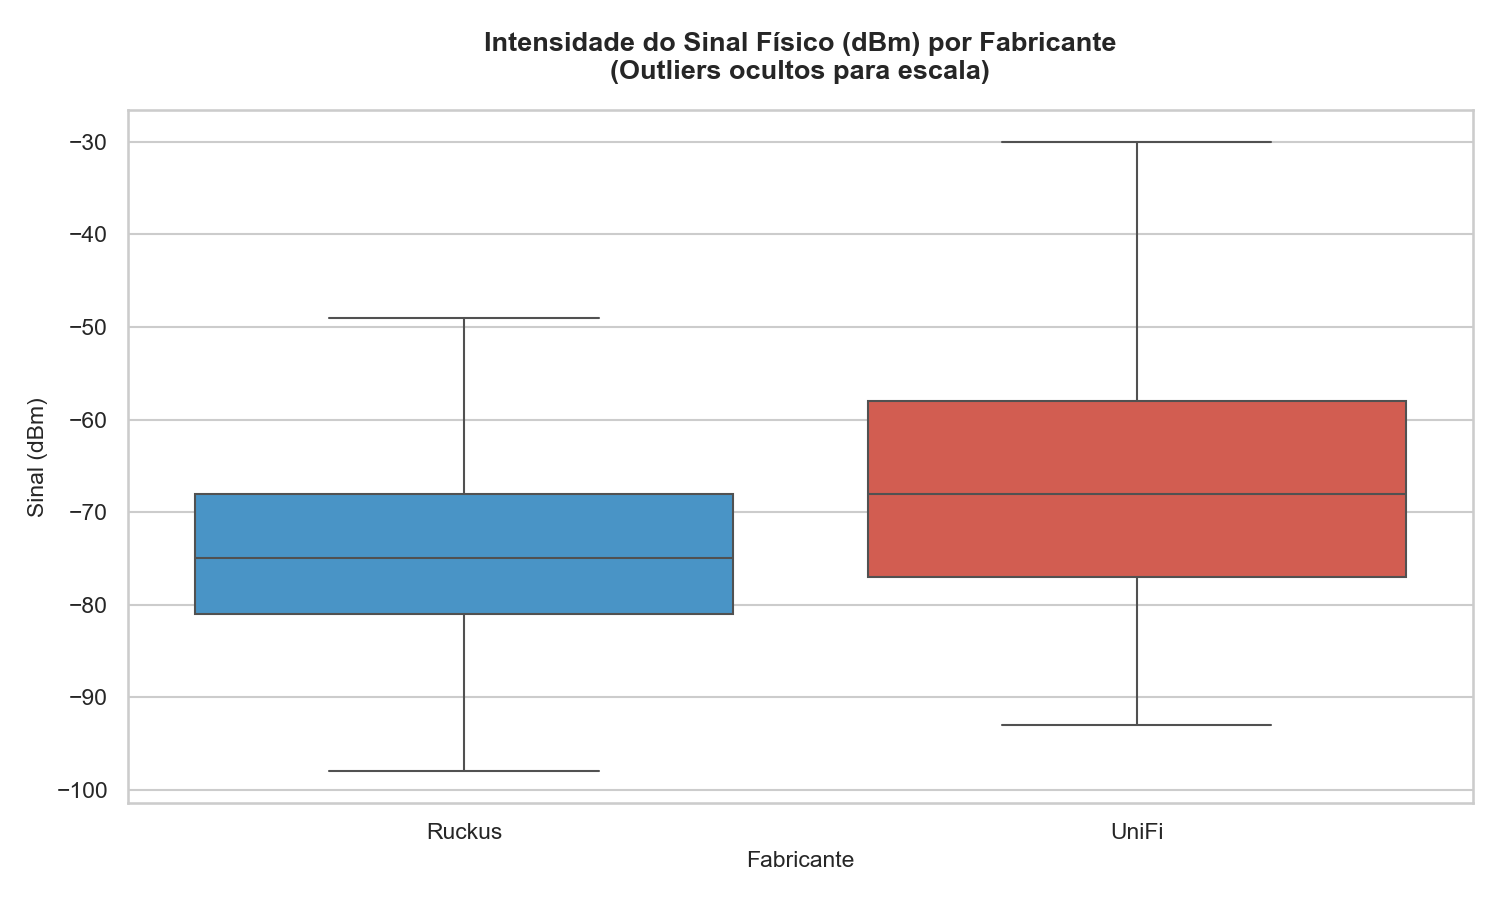
\includegraphics[width=0.85\textwidth]{img/boxplot_rssi_fabricante.png}
  \caption{Boxplot RSSI por Fabricante}
  \label{fig:boxplot_rssi_fabricante_png}
\end{figure}

\begin{itemize}
  \item \textbf{Ruckus}: Média de `-73.83 dBm`, Mediana `-75.00 dBm`.
  \item \textbf{UniFi}: Média de `-67.08 dBm`, Mediana `-68.00 dBm`.
  \item Os resultados sugerem uma cobertura de sinal física coerente para os clientes de ambas as marcas no cenário analisado, com a maioria das amostras se situando em uma faixa saudável de RF.
\end{itemize}

\subsubsection{Histograma de Densidade de Sinal}
O histograma apresenta a densidade de ocorrência de potência de sinal nos logs coletados.

\begin{figure}[H]
  \centering
  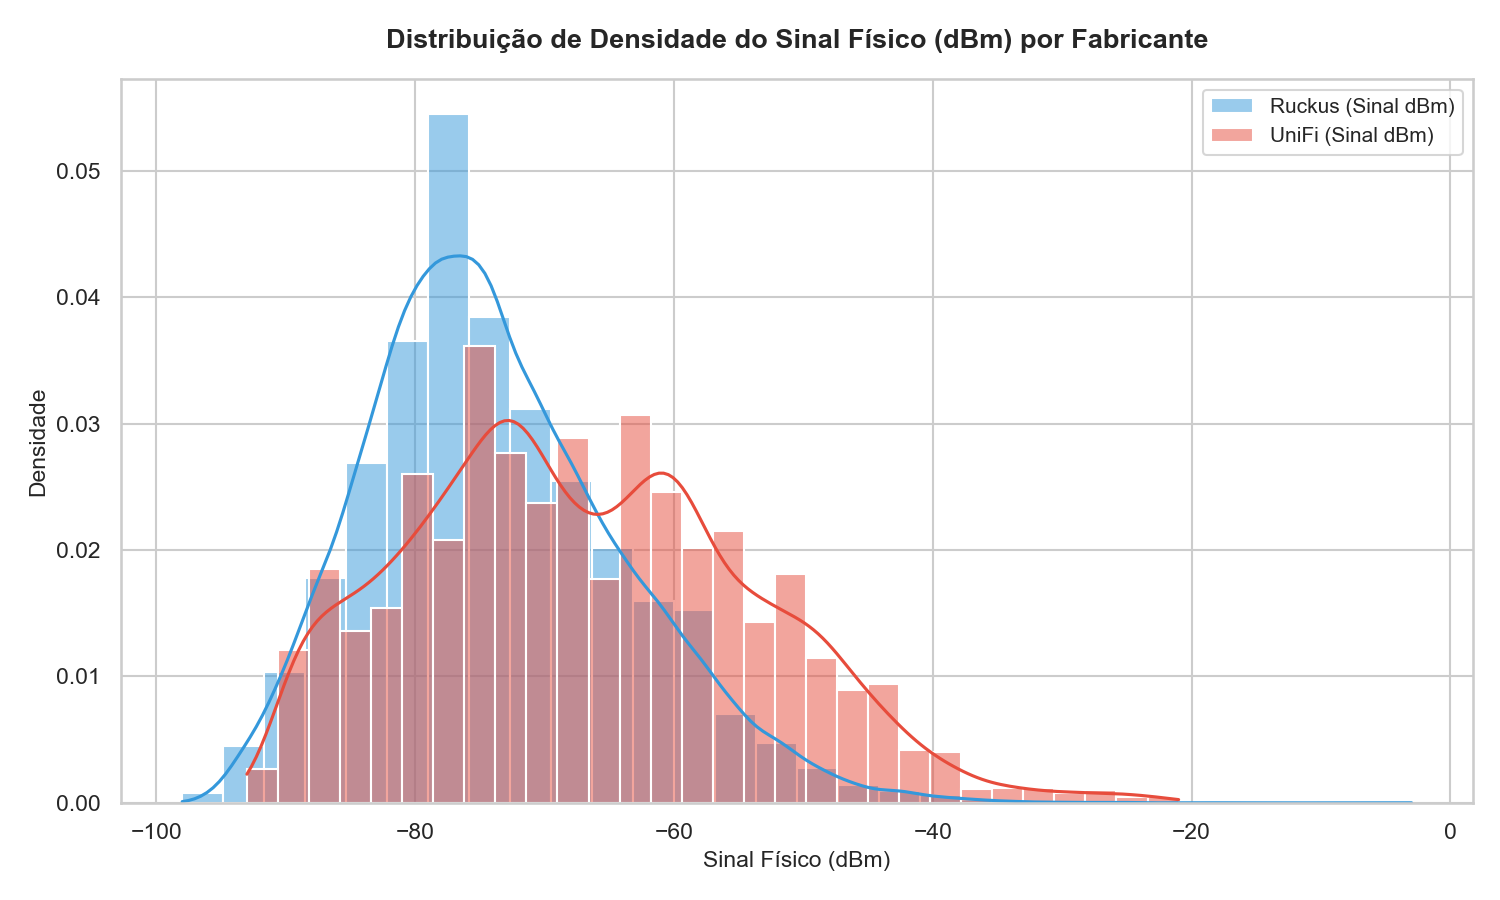
\includegraphics[width=0.85\textwidth]{img/histograma_rssi.png}
  \caption{Histograma RSSI}
  \label{fig:histograma_rssi_png}
\end{figure}

\begin{itemize}
  \item O gráfico demonstra que a UniFi possui uma distribuição de sinal com menor variabilidade (concentrada em torno de -67 dBm), enquanto a Ruckus apresenta maior amplitude e dispersão das conexões ao longo do dia.
\end{itemize}


\subsection{Utilização de Canais por Fabricante}

O histograma de utilização de canais apresenta a contagem de registros em cada frequência de operação.

\begin{figure}[H]
  \centering
  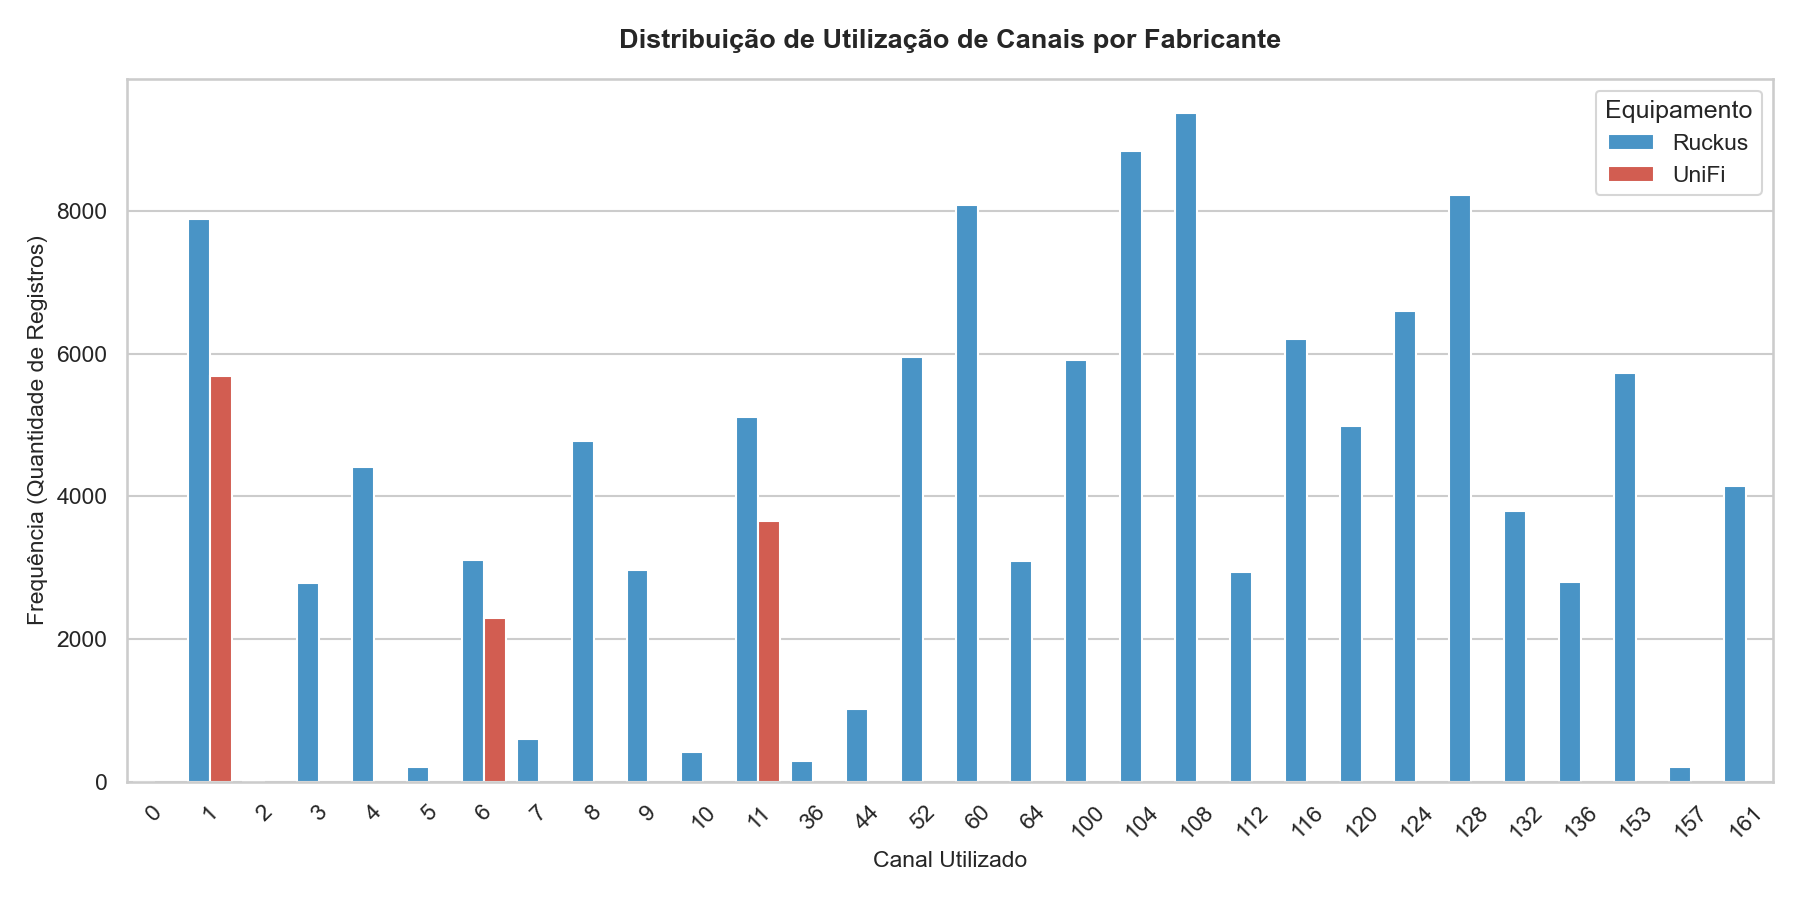
\includegraphics[width=0.85\textwidth]{img/histograma_canais.png}
  \caption{Histograma de Canais}
  \label{fig:histograma_canais_png}
\end{figure}

\begin{itemize}
  \item \textbf{2.4 GHz}: Ambas as marcas concentram o tráfego nos canais não sobrepostos `1`, `6` e `11`, validando as boas práticas de planejamento de RF adotadas no campus.
  \item \textbf{5 GHz}: A Ruckus apresenta uma alocação de espectro mais ampla e distribuída (como canais `36`, `52`, `60`, `104`, `112`, `120`, `128`, `149`), o que reduz interferência co-canal em células adjacentes.
\end{itemize}


\subsection{Quantidade de Clientes Conectados por AP}

Este histograma ilustra a densidade de clientes associados simultaneamente a cada Access Point.

\begin{figure}[H]
  \centering
  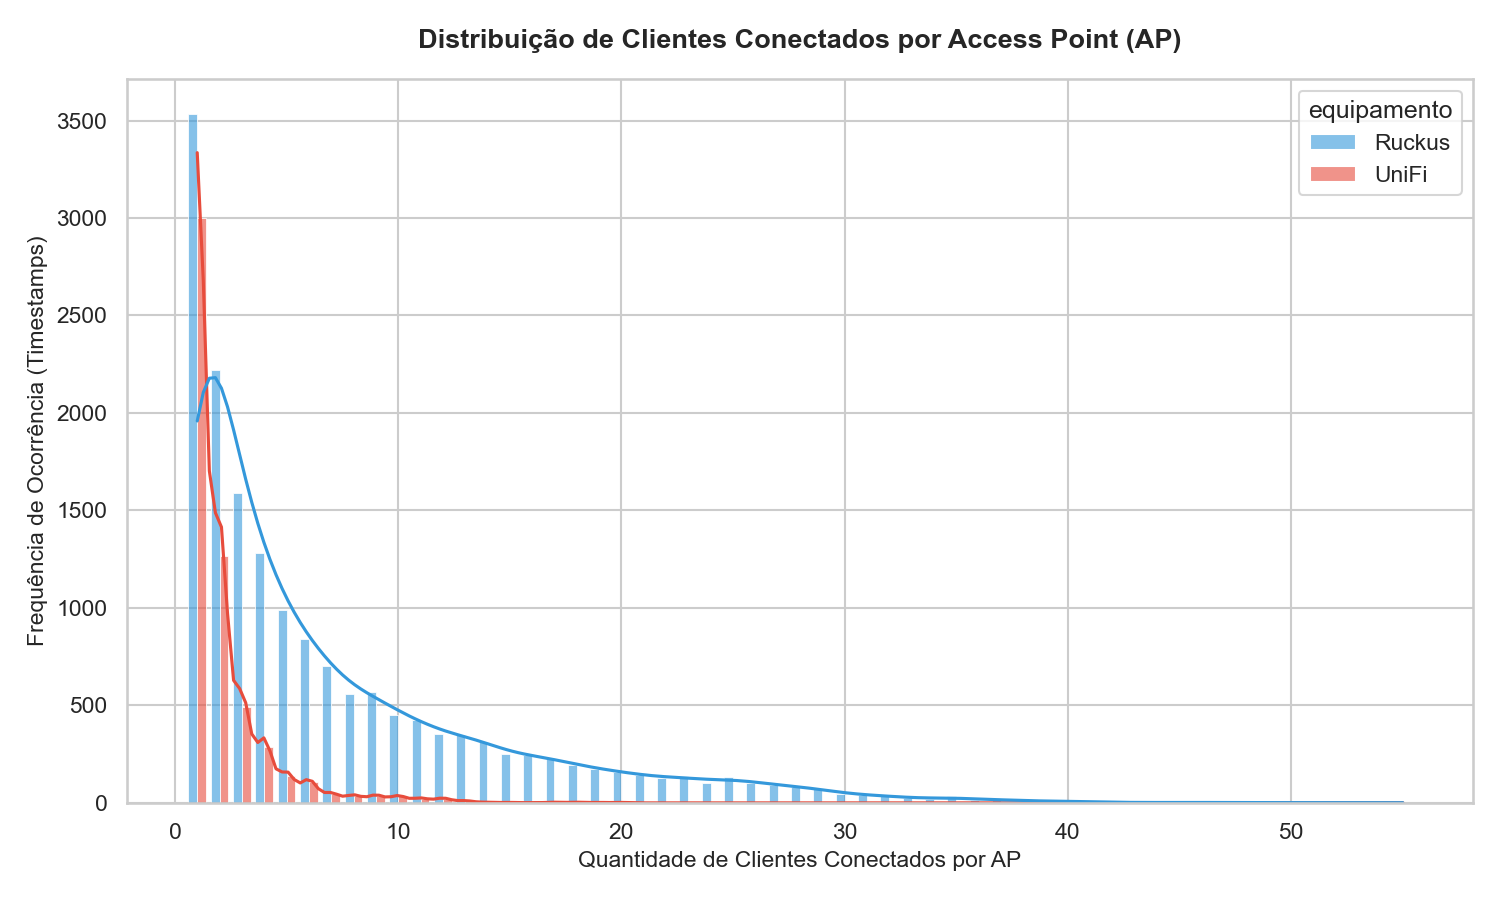
\includegraphics[width=0.85\textwidth]{img/histograma_clientes_por_ap.png}
  \caption{Histograma Clientes por AP}
  \label{fig:histograma_clientes_por_ap_png}
\end{figure}

\begin{itemize}
  \item \textbf{UniFi}: Exibe perfil de baixa carga (maior parte dos registros possui entre 1 e 5 clientes simultâneos por rádio).
  \item \textbf{Ruckus}: Exibe maior flexibilidade de densidade, suportando APs com cargas significativamente mais robustas de concorrência, o que condiz com o posicionamento de alta densidade da marca.
\end{itemize}


\subsection{Análise de Desempenho e Qualidade de Enlace por Banda}

\subsubsection{Throughput por Banda}
O boxplot compara o consumo de throughput entre as bandas de 2.4 GHz e 5 GHz.

\begin{figure}[H]
  \centering
  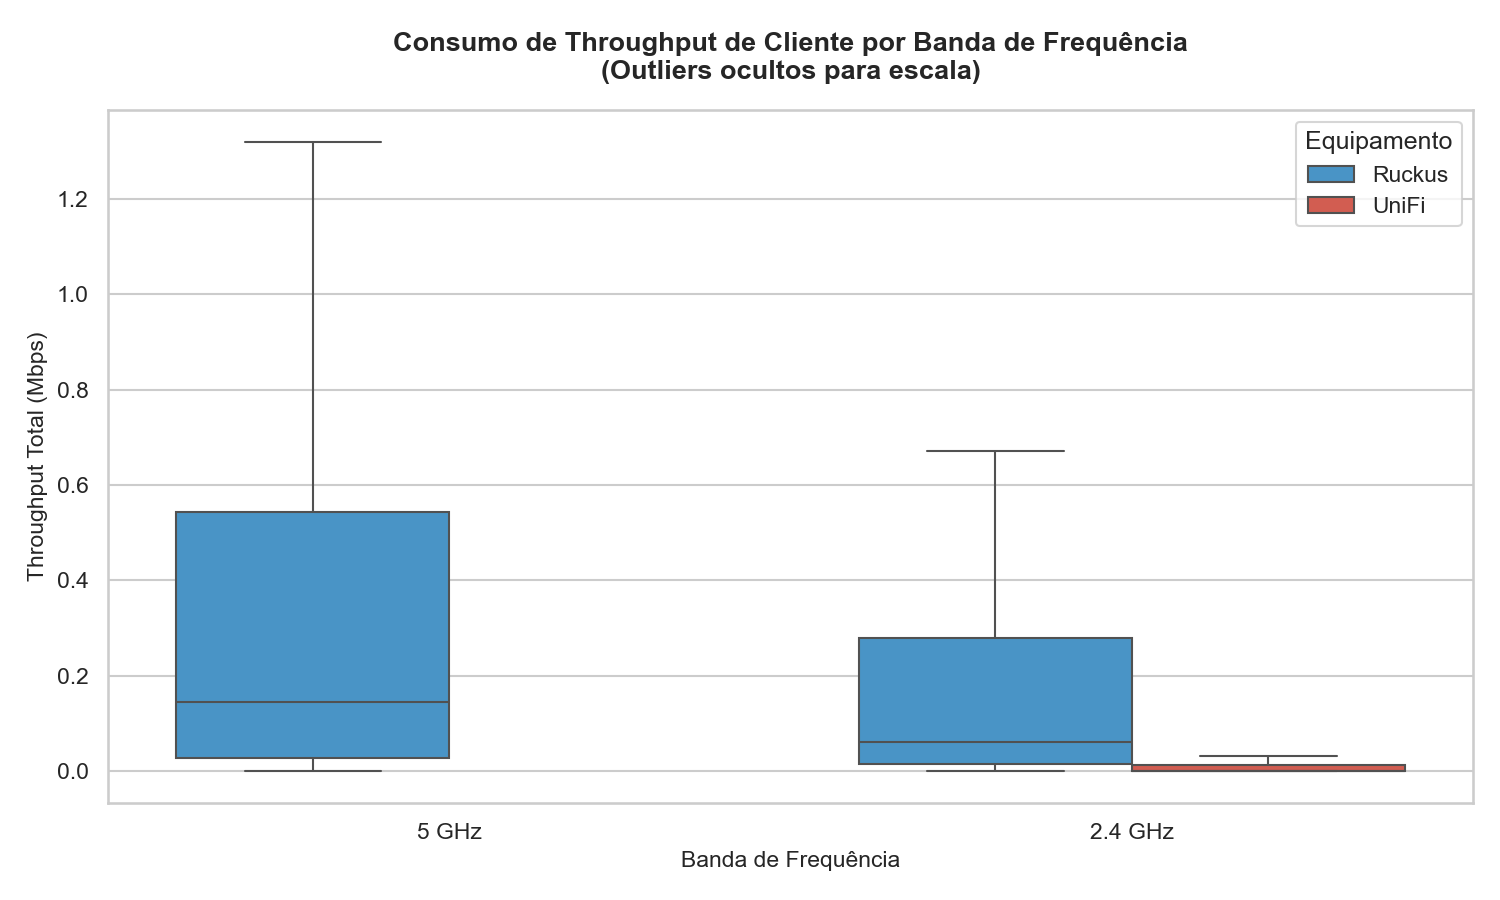
\includegraphics[width=0.85\textwidth]{img/boxplot_throughput_banda.png}
  \caption{Boxplot Throughput por Banda}
  \label{fig:boxplot_throughput_banda_png}
\end{figure}

\begin{itemize}
  \item Como esperado teoricamente, a banda de \textbf{5 GHz} oferece vazão e capacidade física superior para ambas as marcas, superando a banda de \textbf{2.4 GHz} que possui limitações inerentes de modulação e largura de canal.
\end{itemize}

\subsubsection{Retransmissões por Banda}
O boxplot compara a ocorrência de retransmissões físicas ou estimadas.

\begin{figure}[H]
  \centering
  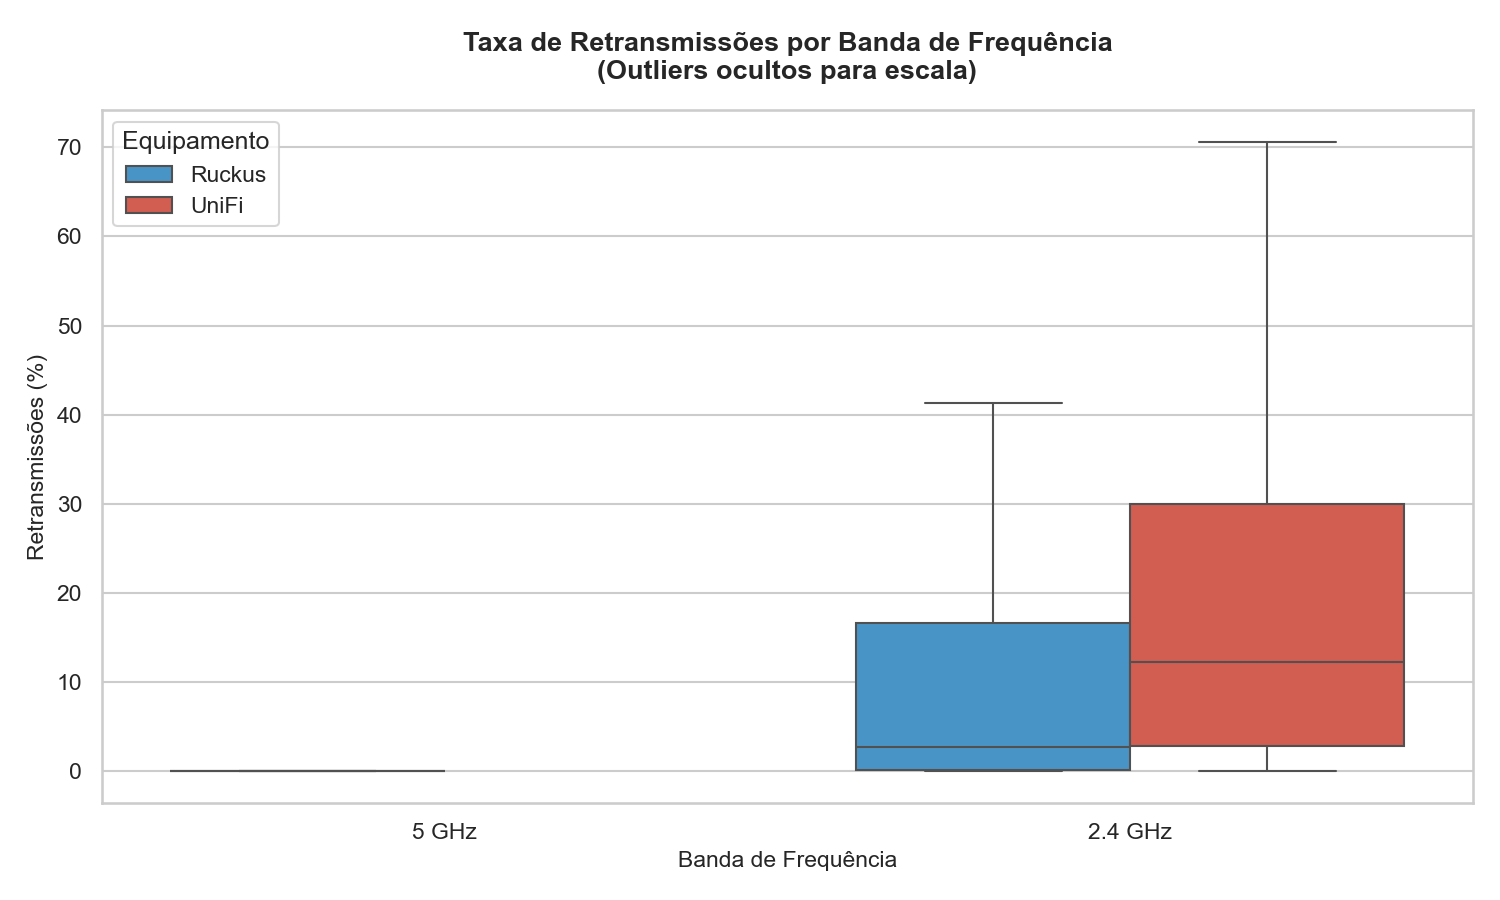
\includegraphics[width=0.85\textwidth]{img/boxplot_retransmissoes_banda.png}
  \caption{Boxplot Retransmissões por Banda}
  \label{fig:boxplot_retransmissoes_banda_png}
\end{figure}

\begin{itemize}
  \item A banda de \textbf{2.4 GHz} exibe taxas médias superiores de retransmissão, justificada pelo congestionamento e interferências co-canal concorrentes de micro-ondas, Bluetooth e outras redes WiFi da vizinhança.
\end{itemize}


\subsection{Distribuição de Throughput Agregado por AP}

Este gráfico apresenta a soma da vazão ativa de todos os clientes associados a cada um dos APs mapeados, permitindo identificar o nível de carregamento individual de tráfego por antena.

\begin{figure}[H]
  \centering
  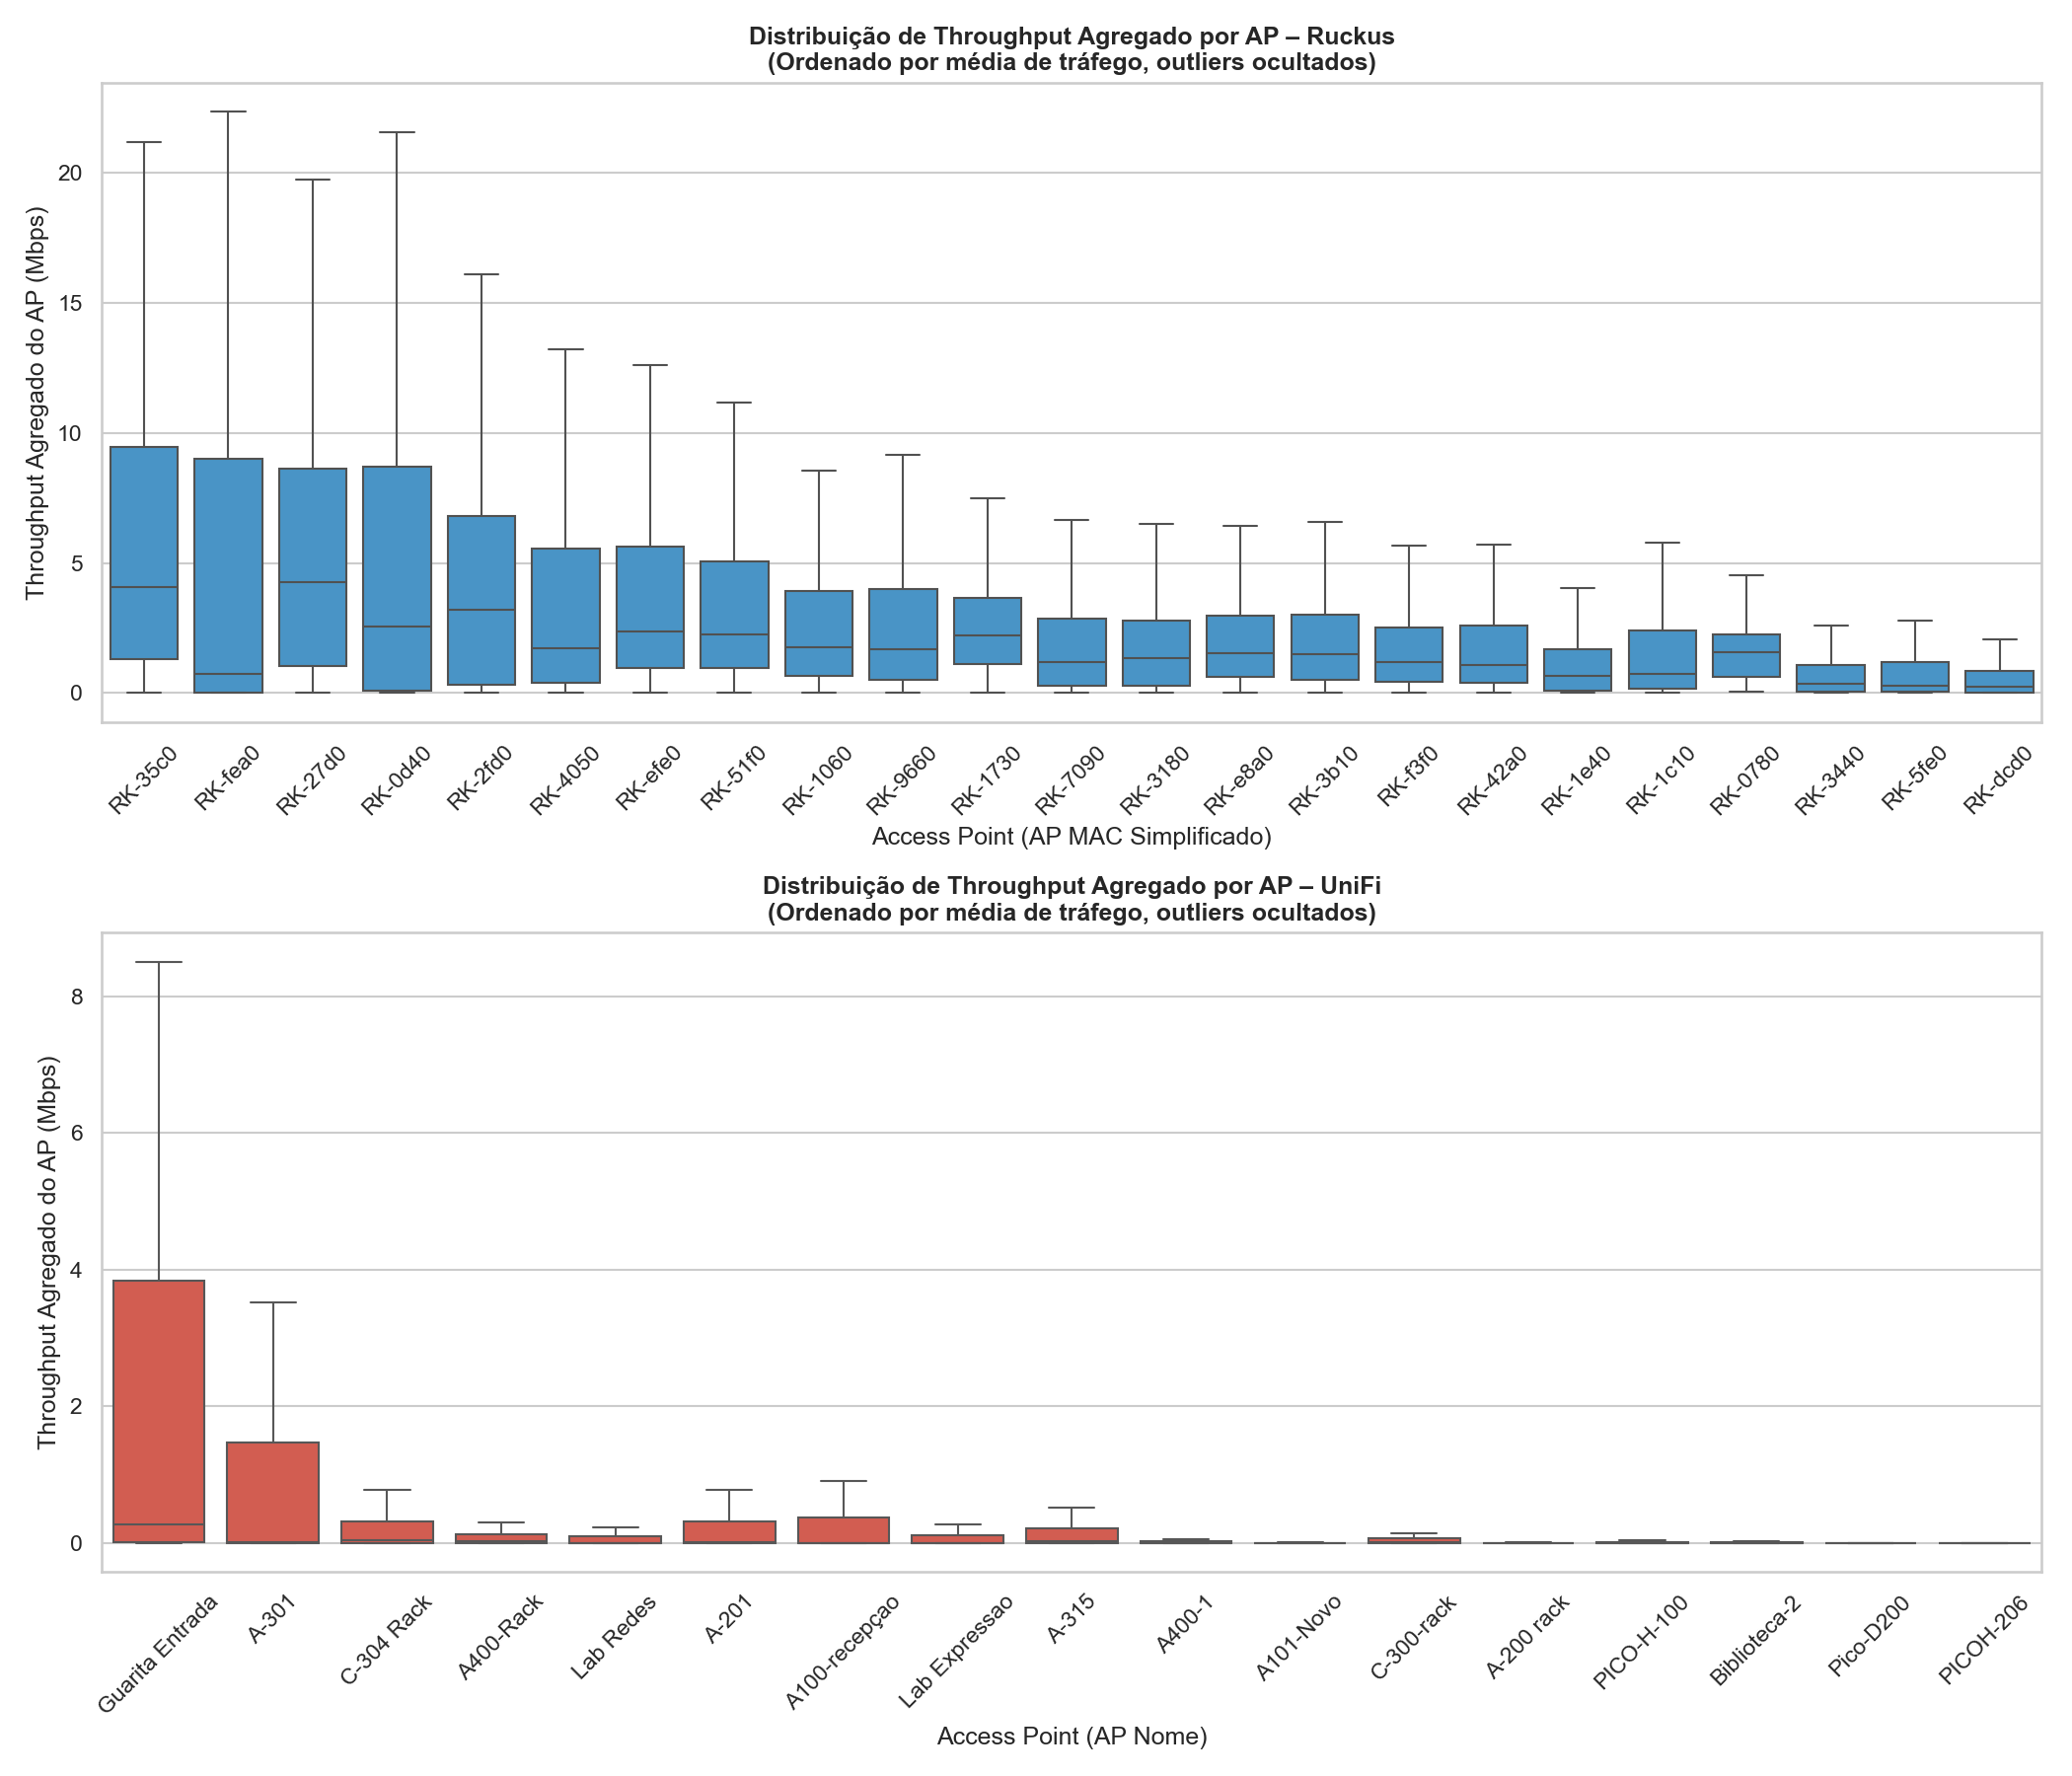
\includegraphics[width=0.85\textwidth]{img/boxplot_throughput_por_ap.png}
  \caption{Boxplot Throughput por AP}
  \label{fig:boxplot_throughput_por_ap_png}
\end{figure}

\begin{itemize}
  \item \textbf{Ruckus (AP MAC Simplificado)}: Apresenta maior amplitude e níveis superiores de vazão somada (vários APs superando médias de 5 a 10 Mbps de tráfego agregado ativo, com picos de consumo expressivos). Para melhor visualização, os endereços MAC longos do Ruckus foram simplificados no formato `RK-XXXX` (onde `XXXX` são os 4 dígitos finais do MAC).
  \item \textbf{UniFi (AP Nome)}: Mostra distribuições de vazão agregada concentradas próximas de zero (com médias inferiores a 2 Mbps). Isso indica que a maioria dos APs da UniFi operaram com carga de dados muito baixa durante o período amostrado, corroborando a ociosidade do ambiente.
\end{itemize}


\subsection{Distribuição Temporal de Clientes Únicos por Fabricante e Dia}

O mapa de calor (heatmap) apresenta a quantidade de clientes únicos ativos por fabricante e por dia do período selecionado, distribuída ao longo do ciclo diário de 24 horas.

\begin{figure}[H]
  \centering
  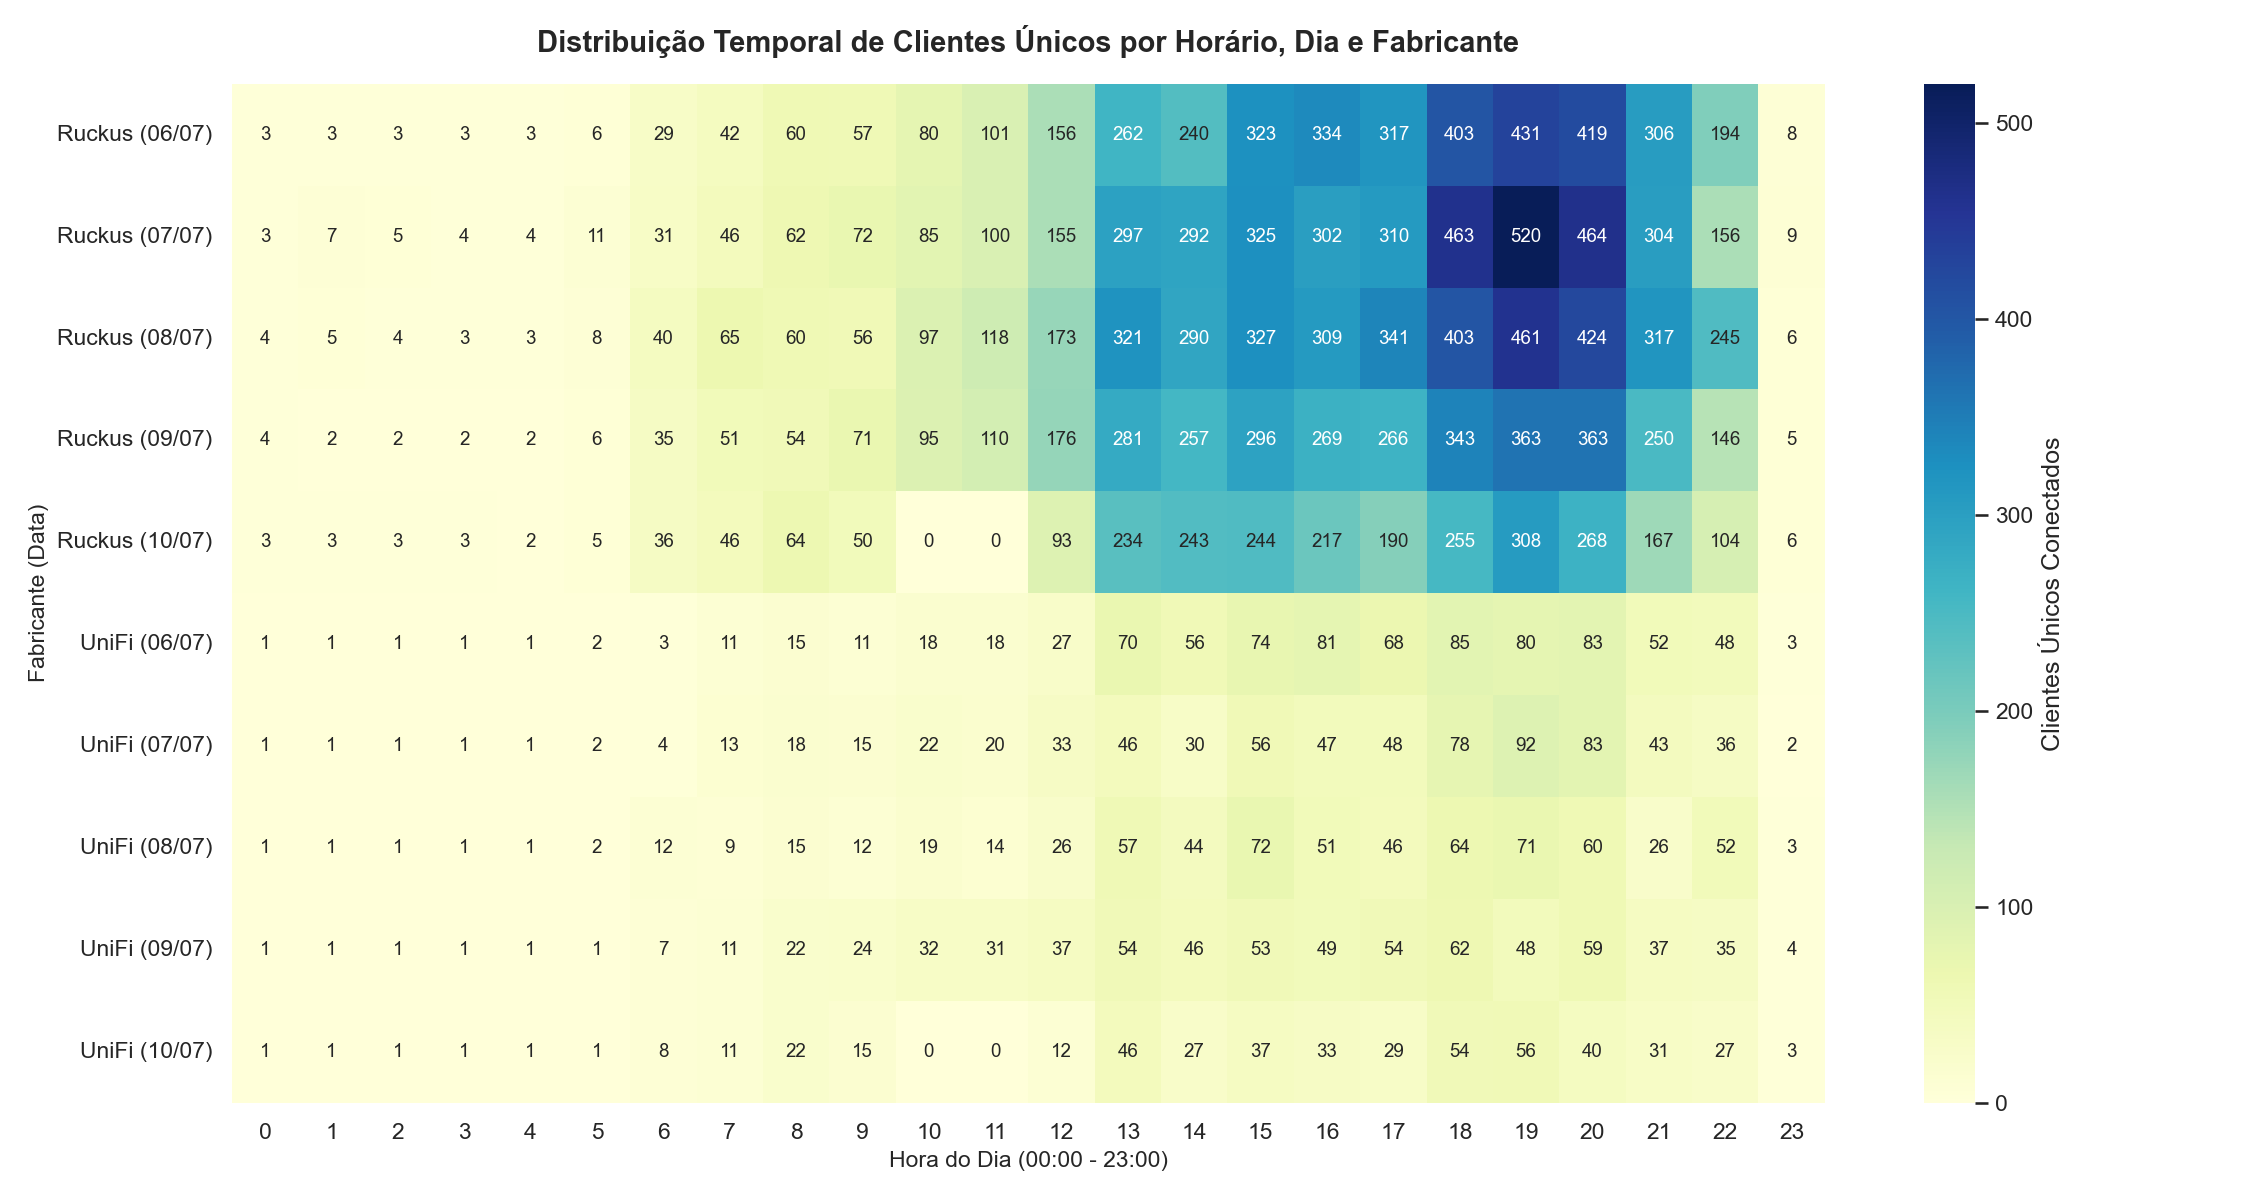
\includegraphics[width=0.85\textwidth]{img/heatmap_horario_clientes.png}
  \caption{Heatmap de Clientes Únicos}
  \label{fig:heatmap_horario_clientes_png}
\end{figure}

\begin{itemize}
  \item O gráfico sugere uma \textbf{rotina cíclica de uso da rede} que se repete de forma semelhante ao longo dos dias: o volume de clientes únicos ativos inicia uma curva ascendente a partir das \textbf{08:00}, atinge os maiores patamares no horário comercial/acadêmico (especialmente entre \textbf{14:00} e \textbf{18:00}) e entra em declínio progressivo nas primeiras horas da noite, reduzindo-se drasticamente durante a madrugada.
  \item \textbf{Picos de Clientes}:
  \item No ambiente Ruckus, o pico de clientes únicos em uma única hora ocorreu no dia \textbf{07/07} às \textbf{19:00}, registrando \textbf{520} dispositivos.
  \item No ambiente UniFi, o pico de clientes únicos ocorreu no dia \textbf{07/07} às \textbf{19:00}, registrando \textbf{92} dispositivos.
  \item Os resultados indicam uma concentração consistentemente maior de dispositivos na infraestrutura Ruckus para todos os dias do período em comparação com a UniFi, o que sugere maior adensamento de usuários sob essa rede no campus observado.
\end{itemize}

